\subsection{Optimizers}

In a very simplistic gradient descent algorithm, a random (or predetermined) initial point, $x_0$, is chosen and then each subsequent value $x_{t+1}$ is determined with the following general updating rule:
\begin{center}
$x_{t+1} = x_t - \alpha_t \nabla F(x_t) $
\end{center}
where $F(x_t)$ is the function to be minimized and $\alpha_t$ is the step length. Thus, the next chosen point, $x_{t+1}$, is found by moving in the direction of the negative gradient. In application to neural networks, the function $F(x_t)$ is known as the loss function, and the gradient of this loss function is used to update its layer weights, $w_i$. These layer weights are used to then predict outputs. The loss function is typically in the form of $L(w_i,x_i,y_i,\hat y_i)$, where $(x_i,y_i)$ are individual training samples (input and output), and $\hat y_i$ is the neural networks prediction from the training input. These training samples are taken from a set of training data, $\textbf{\textit{D}}$, where
\begin{center}
$\textbf{\textit{D}} = \{(x_i,y_i),...,(x_k,y_k)\}$
\end{center}
and the objective function is in the form:
\begin{center}
$\min\limits_{x_i \in X} L(w_i,x_i,y_i,\hat y_i)$
\end{center}
Since the objective function shown above is typically non-convex and can have many pseudo-optimal solutions, direct solutions of the cost function are not feasible. Instead, gradient descent algorithms can be used to find a set of optimal parameters for this minimization problem, where an initial set of weights, $w_0$ are chosen and the update rule becomes:
\begin{center}
$x_{t+1} = x_t - \eta_t \nabla L_t(w_i,x_i,y_i,\hat y_i)$
\end{center}
where $\eta_t$ is step length (called the learning rate), and $\nabla L_t$ is gradient at the current time step. This update rule is very simplistic though, and in practical usage a more complicated function, known as an optimizer, is typically used to improve the efficacy of these update steps.

\subsubsection{SGD Algorithm}
The SGD algorithm is one of the most common (and basic) gradient descent algorithms used in neural network training. The adapted algorithm for mini-batches is as follows:
\vspace{14pt}
\begin{minipage}[b]{.48\textwidth}
\begin{algorithm}[H]\small
	\caption{SGD \cite{SGD}}
	\label{alg:SGD}
	\begin{algorithmic}
		\STATE {\bfseries Input:} Training samples: \textbf{\textit{X}} \subset $\{x_t\}_{t=1}^T$, $x_t \in \mathbb{R}^d$, $\{\eta_t\}_{t=1}^T$, $\epsilon>0$
		\vspace{4pt}
		\FOR{$t=1,...,T$}
		    \vspace{3pt}
		    \STATE Randomly sample point $(x_t,y_t)$ from \textbf{\textit{X}}
		    \vspace{3pt}
		    \STATE Compute $\hat y_t$ from current network weights, $w_t$
		    \vspace{3pt}
		    \STATE Compute $\nabla L_t(w_t,\tilde x_{k},\tilde y_k,\hat y_k)$
		    \vspace{3pt}
		    \STATE $w_{t+1}^{(i)} = w_{t}^{(i)} + \eta_t (\nabla L_{t}^{(i)} + \epsilon) \: \forall  i$
		\vspace{3pt}
		\ENDFOR
	\end{algorithmic}
\end{algorithm}
\end{minipage}\hfill
\vspace{-8pt}
In the update step, the $i$ superscript signifies the operation is performed individually across all layer weights in the model. The addition of the extra hyperparameter $\epsilon$ is a small number chosen to prevent updates of zero magnitude.

In summary, the SGD algorithm is similar to the vanilla GD algorithm outline before, except that the order of the input training data is randomly selected. A popular extension of this algorithm is to delay the update to the weights by averaging the loss function calculation across several training sample, in a process called mini-batch training. The advantage behind performing mini-batches as opposed to weight updates after individual samples is for two reasons:
\vspace{4pt}
\begin{enumerate}
    \item Averaging the gradient across samples has been shown to lower the chances of over-fitting. \cite{Masters2018RevisitingSB}
    \item Weight-updates can be performed in a parallel / asynchronous setting, where work can be distributed across individual processors and summed at the end. This is because weight-updates are performed after several samples have been run, instead of after each sample.
\end{enumerate}
\vspace{3pt}

Mini-batch SGD has been shown to easily converge many moderately sized neural networks, but proves to be less than optimal when the network becomes large or when there is large variance sample to sample. Any other gradient descent-based algorithm can implement this strategy, and it is so widely used in practice that going forward it will be assumed that all other optimizers are implemented in a "mini-batch" fashion.
\subsubsection{LARS optimizer}

The LARS optimizer (short for Layer-wise Adaptive Rate Scaling), developed and outlined by You et al. in \cite{ginsburg2018large}, improves upon the previous SGD algorithm by introducing a normalization calculation done on each update step. This normalization involves scaling the effective learning rate with respect to the individual neural network layers. They found that the ratio of $||w_t^{(l)}||$ ($l_2$ norm of the current weights at layer $l$) to $||L_t^{(l)}||$ ($l_2$ norm of the loss function at layer $l$) varied tremendously from the initial to final layers. They proposed a singular addition to traditional gradient descent: scale the learning rate $\eta_t$ by a second parameter called the "trust" or "lars" coefficient ($\gamma$) and by the ratio $\frac{||w_t^{(l)}||}{||\nabla L(w_t^{(l)})||}$. They hypothesized that training would substantially improve for deep neural networks due to the extra normalization. They proved this was the case for the ResNet-50 model even when trained with extremely large batch sizes (greater than 32k)\cite{ginsburg2018large}. This holds large relevance as being able to increase the batch size allows for more parallel/distributed training, better utilizing larger amounts of computing ability. An outline of the algorithm in the case of SGD with LARS is as follows:
\begin{minipage}[b]{.48\textwidth}
\begin{algorithm}[H]\small
	\caption{SGD with LARS \cite{ginsburg2018large}}
	\label{alg:lars}
	\begin{algorithmic}
	    \vspace{3pt}
		\STATE {\bfseries Input:}Training samples: \textbf{\textit{X}} \subset $\{x_t\}_{t=1}^T$, $x_t \in \mathbb{R}^d$, $\{\eta_t\}_{t=1}^T$, $\epsilon>0$
		$x_i \in \mathbb{R}^d$, LARS coefficient $\gamma <1$
		\vspace{4pt}
		\FOR{$t=1,..., T$}
		\vspace{3pt}
		    \STATE Randomly sample point $(x_t,y_t)$ from \textbf{\textit{X}}
		    \vspace{3pt}
		    \STATE Compute $\hat y_t$ from current network weights, $w_t$
		    \vspace{3pt}
		    \STATE Compute $\nabla L_t(w_t, x_{k}, y_k,\hat y_k)$
		    \vspace{3pt}
        \STATE $\lambda_t^l \gets \frac{||w_t^l||}{||\nabla L(w_t^l)||}$ (local LR across each layer $l$)
        \vspace{3pt}
		    \STATE $w_{t+1}^{l} = w_{t}^{l} + \eta_t \gamma_t \lambda_t^l(\nabla L_{t}^{l} + \epsilon) \: \forall  l$
        % \STATE $v_{t} = \beta v_{t-1} + \gamma_t\eta(1 - \beta)\lambda^l\nabla L(w_t^l)$ (momentum calculation)
% 		\STATE $v_{t+1}^l = \eta_t  ||w_t^{(i)}||\frac{m_t^{(i)}}{\|m_t^{(i)}\|} $ for all $i \in [h]$
%         \vspace{3pt}
% 		\STATE $w_{t+1} = w_{t} - v_t$ (update weights)
		\vspace{3pt}
		
		\ENDFOR
	\end{algorithmic}
\end{algorithm}
\end{minipage}\hfill%
% \begin{algorithm}[htb!]%[t]
% \begin{algorithmic}
% \STATE {\bf Parameters:} base LR $\gamma_0$, momentum $m$, weight decay $\beta$, LARS coefficient $\eta$, number of steps $T$
% \STATE {\bf Init:} $t = 0, v = 0$. Init weight $w_0^l$ for each layer $l$
% \WHILE {$t < T$ for each layer $l$} 
%         \STATE $g_t^l \gets \nabla L(w_t^l)$   (obtain a stochastic gradient for the current mini-batch)
%         \STATE $\gamma_t \gets \gamma_0 * \left(1 - \frac{t}{T}\right)^2$ (compute the global learning rate)
%         \STATE $\lambda^l \gets \frac{||w_t^l||}{||g_t^l|| + \beta ||w_t^l||}$       (compute the local LR  $\lambda^l$)
%         \STATE $v_{t+1}^l \gets mv_t^l + \gamma_{t+1} * \lambda^l * (g_t^l + \beta w_t^l)$     (update the momentum)
%         \STATE $w_{t+1}^l \gets w_t^l - v_{t+1}^l$ (update the 
%         weights)
% \ENDWHILE
% \end{algorithmic}
%  \caption{Mini-batch SGD with LARS. Example with momentum\label{algo:lars}}
% \end{algorithm}

Weight updates are still also performed across each individual weight, $w_i$, but this superscript was left out for sake of simplicity. It is important to note that there are two key differences between this implementation and traditional SGD:
\begin{enumerate}
    \item The learning rate is now parameterized by the layer number, $l$
    \item The calculation of the trust coefficient, $\lambda^l_t$, is scaled by the LARS coefficient, $\eta$, to apply different magnitudes of LR scaling
\end{enumerate}
\vspace{4pt}

It can be deduced that the performance benefit seen by You et al. was from the normalization of the magnitude of the update step with respect to the layers. In practice, this means that only the direction of the gradient and the current magnitude of the weights is taken into consideration for each update step. It is assumed that this layer-wise normalization allow for deep networks to be trained for higher numbers of iterations with a less likelihood of over-fitting. When applied to the mini-batch case, gradient updates are performed in the same manner, where the gradient updates at each mini-batch are averaged to make a singular update. 

\subsubsection{ADAM optimizer}
Although LARS makes many improvements to traditional SGD algorithms, it still does not incorporate higher-order terms that could benefit each update step. The ADAM optimizer, created by  in \cite{adam}, enhances regular gradient descent algorithms through the addition of two terms and two hyperparameters:
% It introduces exponential moving average on the first and second order of the gradient:
\vspace{-10pt}
\begin{align*}
m_{t} = \beta_{1}m_{t-1}+(1-\beta_{1})g_{t} \\
v_{t} = \beta_{2}v_{t-1}+(1-\beta_{2})g_{t}^2
\end{align*}

The first and second term, $m_{t}$, $v_t$, represent the exponential moving average of the first and second moment of the gradient of the loss function, $g_t$, respectively. The two hyper parameters, $\beta_1$ and $\beta_2$ represent the weighting of the previous and current values. After calculating these two values, there is also a bias correction step:
\begin{align*}
\hat{m}_{t}=\frac{m_t}{1-\beta_1^t} \\
\hat{v}_{t}=\frac{v_t}{1-\beta_2^t}
\end{align*}
\vspace{-10pt}

The addition of these two terms comes from the calculation of the expected value of each moment, which is corrected by dividing the current moment by $(1 - \beta_i^t)$, where t is the current step number. This operation makes $m_t$ and $v_t$ \textit{unbiased estimators} of the first and second moment of the gradient. The algorithm is as follows:
\begin{minipage}[b]{.48\textwidth}
\begin{algorithm}[H]\small
	\caption{ADAM \cite{adam}}
	\label{alg:adam}
	\begin{algorithmic}
% 		\STATE {\bfseries Input:} $x_i \in \mathbb{R}^d$, learning rate $\{\eta_t\}_{t=1}^T$, parameter,  $\epsilon > 0$
		\STATE {\bfseries Input:} Training samples: \textbf{\textit{X}} \subset $\{x_t\}_{t=1}^T$, $x_t \in \mathbb{R}^d$, $\{\eta_t\}_{t=1}^T$, $\epsilon>0$,  $\beta_{1},\beta_{2} \in [0,1)$
		\vspace{3pt}
		\STATE Initialize $m_{0} = 0, v_{0} = 0$
		\FOR{$t=1,...,T$}
		\vspace{3pt}
		\STATE Randomly sample point $(x_t,y_t)$ from \textbf{\textit{X}}
		\vspace{3pt}
		\STATE Compute $\hat y_t$ from current network weights, $w_t$
		\vspace{3pt}
		\STATE Compute $\nabla L_t(w_t, x_{t}, y_t,\hat y_t)$
		\vspace{3pt}
        \STATE $m_{t} = \beta_{1}m_{t-1}+(1-\beta_{1})\nabla L_t$
        \vspace{3pt}
        \STATE $v_{t} = \beta_{2}v_{t-1}+(1-\beta_{2})\nabla L_t^2$
        \vspace{3pt}
        \STATE $\hat{m}_{t}={m_t}/(1-\beta_1^t)$
        \vspace{3pt}
        \STATE $\hat{v}_{t}={v_t}/(1-\beta_2^t)$
        \vspace{2pt}
        \STATE $w_{t+1} = w_{t}-\eta_t\frac{\hat{m}_t}{\hat{v}_t+\epsilon}$
        \vspace{3pt}
		\ENDFOR
	\end{algorithmic}
\end{algorithm}
\end{minipage}\hfill%

The value calculated at the end in the form of $\frac{\hat{m}_t}{\hat{v}_t+\epsilon}$ is also known as the Adam norm. Typical values for $b_1$ and $b_2$ are 0.9 and 0.999 \cite{adam}, which are shown to work effectively across all use cases.

\subsubsection{LAMB optimizer}

The LAMB algorithm, developed by You et al. in \cite{You2020Large} uses ADAM as the base algorithm, and applies the same layer-wise normalization that LARS implements. More specifically, it makes the following adjustments:
\begin{enumerate}
    \item Use the square root of second moment, $\hat v_t$ for normalization and calculation of the Adam norm.
    \item Adopt a parameterization function of the inputs, $\phi(||w_t^{(l)}||)$, for layer-wise normalization
\end{enumerate}

The algorithm is as follows:
\begin{minipage}[b]{.5\textwidth}
\begin{algorithm}[H]\small
	\caption{$LAMB$ \cite{You2020Large}}
	\label{alg:lamb}
	\begin{algorithmic}
		\STATE {\bf Input:}  Training samples: \textbf{\textit{X}} \subset $\{x_t\}_{t=1}^T$, $x_t \in \mathbb{R}^d$, $\{\eta_t\}_{t=1}^T$, $\epsilon>0$,  $\beta_{1},\beta_{2} \in [0,1)$, scaling function $\phi(w_t)$
		\vspace{3pt}
		\STATE Set $m_{0} = 0$, $v_{0} = 0$
		\vspace{3pt}
		\FOR{$t=1,...,T$}
		\STATE Randomly sample point $(x_t,y_t)$ from \textbf{\textit{X}}
		\vspace{3pt}
		\STATE Compute $\hat y_t$ from current network weights, $w_t$
		\vspace{3pt}
		\STATE Compute $\nabla L_t(w_t, x_{t}, y_t,\hat y_t)$
		\vspace{3pt}
		\STATE $m_{t} = \beta_{1}m_{t-1}+(1-\beta_{1})\nabla L_t$
        \vspace{3pt}
        \STATE $v_{t} = \beta_{2}v_{t-1}+(1-\beta_{2})\nabla L_t^2$
        \vspace{3pt}
        \STATE $\hat{m}_{t}={m_t}/(1-\beta_1^t)$
        \vspace{3pt}
        \STATE $\hat{v}_{t}={v_t}/(1-\beta_2^t)$
        \vspace{3pt}
		\STATE Compute trust ratio $r_t = \frac{m_t}{\sqrt{v_t} + \epsilon}$
		\vspace{3pt}
		\STATE $w_{t+1}^{(l)} = w_{t}^{(l)} - \eta_t \frac{\phi||w_t^{(l)}||)}{||r_t^{(l)} + \lambda w_t^{(l)}||} (r_t^{(l)} + \lambda w_t^{(l)})$
		\ENDFOR
	\end{algorithmic}
\end{algorithm}
\end{minipage}

Choices for the parameterization function $\phi$ can include a simple $\phi(z) = z$, or can be more complex and perform ceiling/floor operations. You et al. found that either of these choices resulted in similar performance\cite{You2020Large}. The inclusion of layer-based scaling should allow for the ability to perform larger batch sizes with minimal negative effect (similar to LARS). The inclusion of moment calculations should allow for much faster minima convergence, as shown by previous researchers with the advent of Adam \cite{adam}. It is hypothesized that the pairing of these two greatly improves upon the traditional LARS + SGD approach mentioned previous in terms of training speed and efficiency. 
\subsection{Study Cases' Models}

\subsubsection{Image Classification}

\begin{enumerate}[start=1,label={\bfseries\arabic*:}]
    \item A set of convolution layer and pooling layer to compress the image
    \item Another set of convolution layer and pooling layer to further compress the data
    \item Two fully connected layers after flattens the data to do the neural network training.
    \end{enumerate}
    
%The first part of the network is a straightforward CNN model and it uses Relu as activation function. It consists of two consecutive convolution layer and pooling layer in order to capture the potential features of the images. The second part of the network flattens the condensed image and then uses two fully connected layer to do the classification.

The cost function is calculated by negative log likelihood loss:
\begin{align*}
    J(y) = -log(y) 
\end{align*}

Note there is only one term in the loss function per data, which is the negative log likelihood of the predicted value of the true label. This negative loss likelihood function works better when the neural network model has a high confidence at the correct class. When training in batch, the cost function per batch is the sum of the individual negative log likelihood costs.

\subsubsection{QA System}


The model employed for QA understanding system here is called Document retriever Question Answering (DrQA) as illustrated in Figure~\ref{fig:DrQA}.  Starting from the top:
\begin{enumerate}[start=1,label={\bfseries\arabic*:}]
    \item According to Lee et al. \cite{Lee}, the questions and context can be aligned to build respective embedding of:     \vspace{5pt}

    \begin{center} $f_{align} = \sum_j \alpha_{i, j} E(q_j)$. \end{center}
    \vspace{5pt}
    Where $\alpha$ is single dense layer with relu non-linearity and $E()$ represents the glove embeddings. This layer help initialize what portion of the context is more important or relevant with respect to the question.
    
    \item In order to understand the representation of these glove and aligned paragraphs, these are passed to stacked bi-LSTM \cite{biLSTM}. LSTM is expressed as: 
    \vspace{5pt}
    \begin{center}
    $u_t = \sigma(W_u x_t + U_u h_{t-1} + b_u)$ \\
    $f_t = \sigma(W_f x_t + U_f h_{t-1} + b_f)$  \\
    $g_t = tanh(W_g x_t + U_g h_{t-1} + b_g)$  \\
    $o_t = \sigma(W_o x_t + U_o h_{t-1} + b_o)$  \\
    $c_t = f_t c_{t-1} + u_t g_t$ \\
    $h_t = o_t tanh(c_t)$
    \end{center}
        \vspace{5pt}

    where $u, f, g, o$ are  respectively update/input, forget, cell, and output gates. $c_t$ is the cell at time $t$ and $\sigma(\cdot)$ is the sigmoid function. 
    
    \item Then the importance of each word in the question is calculated through Linear Attention layer as $b$ below with $w$ as a trainable weight vector:
        \vspace{5pt}

    \begin{center} 
    $b_j = \frac{e^{w \cdot q_j}}{\sum_{j'}e^{w\cdot q_{j'}}}$
    \end{center}
        \vspace{5pt}

    \item Finally, to predict the accurate answer's span tokens, there are two bilinear classifiers to respectively predict the probabilities of start and end tokens of the span: 
        \vspace{5pt}

    \begin{center} 
    $P_{start}(i) \propto e^{p_iW_sq}$ \\
    $P_{end}(i) \propto e^{p_iW_eq}$
    \end{center}
    
    
\end{enumerate}


\begin{figure}[!t]
    \centering
    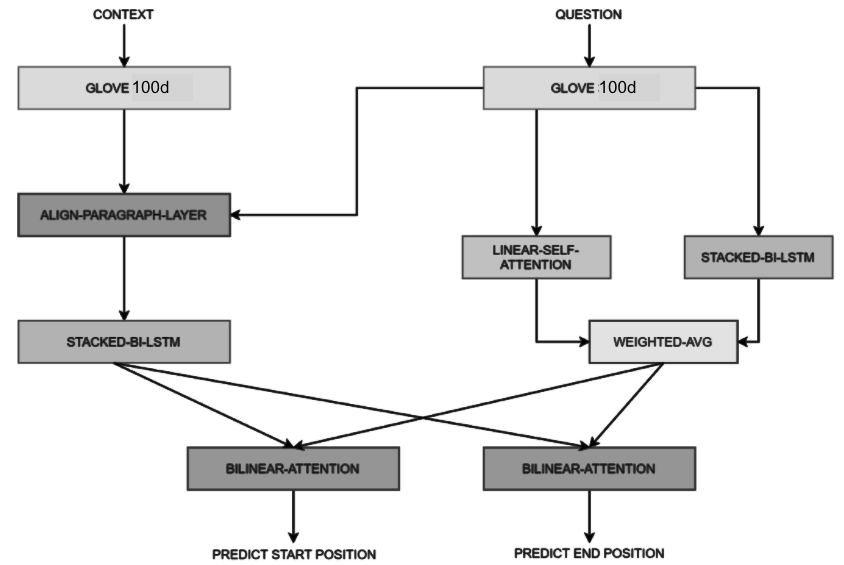
\includegraphics[width=\linewidth]{img/DrQA.png}
    \caption{Document Reader model architecture part of DrQA \cite{DrQA, drqa_architecture}}
    \label{fig:DrQA}
\end{figure}

% As the name suggested, the model included Document Retriever and Document Reader: 




\subsubsection{Speech to Text}

The model is a variant of the Deep Speech 2 model with the aid of Residual CNN (Res-CNN)

% Model is similar to Deep Speech 2, model, but first preprocesses the data into a spectrogram, then these are fed into 3 Residual CNN blocks to extract feature vectors of length 500 from the audio data, and a set of 3 bidirectional GRU-RNN layers to translate the extracted features into an intermediate output vector, which is fed into a fully connected layer, then a softmax, then a 28 long vector mapping of probabilities of corresponding letters or symbols.

\begin{figure*}[!t]
    \centering
    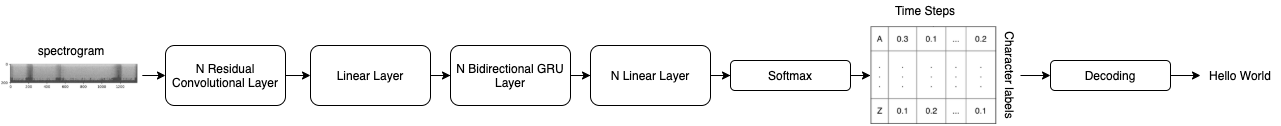
\includegraphics[width=\linewidth]{img/speech.png}
    \caption{A variant of Deep Speech 2 architecture that utilizes Res-CNN.}
    \label{fig:deepSpeech}
    \vspace{-10pt}
\end{figure*}

\begin{enumerate}[start=1,label={\bfseries \arabic*:}]
    \item Residual network consists of stacked ``residual units'' inspired by He et al. \cite{resnet} but with layer norm to learn the audio features expressed as:
        \vspace{5pt}

    \begin{center}
    $x_{l + 1} = ReLU(h(x_l) + F(x_l, W_l))$ \\
    \end{center}
    \vspace{5pt}
    
    \item A fully connected layer to compress the model representation before passing it over. 
    
    \item Bidirectional GRU-RNN \cite{biGRURNN} is then utilized to leverage the features to learn the representation of the audio's spectrogram frames before the current step and after it as well. 
        \vspace{5pt}

    \begin{center}
    
    $u_t &= \sigma(W_u x_t + U_u h_{t-1} + b_u)$ \\
    $r_t &= \sigma(W_r x_t + U_r h_{t-1} + b_r)$ \\
    $\tilde{h}_t &= f(W_h x_t + r_t \circ U_h h_{t-1} + b_h)$ \\
    $h_t &= (1 - u_t) h_{t-1} + u_t \tilde{h}_t$

    \end{center}
        \vspace{5pt}

    $u$ and $r$ represent the \emph{update} and \emph{reset} gates respectively. This is slightly different from the standard GRU in that the hidden state $h_{t-1}$ is multiplied by $U_h$ prior to scaling by the reset gate. This allows for all operations on $h_{t-1}$ to be computed in a single matrix multiplication. Moreover, Amodei et al. \cite{Amodei} found similar performance for $tanh$ and clipped-ReLU for nonlinear transformation so clipped-ReLU \cite{clippedReLU} is picked for simplicity and uniformity with the rest of the network.

    
    \item A final fully connected layer takes the inputs from the feature analysis and applies weights to predict the correct label.
    
    \item A Gaussian Error Linear Unit (GELU) activation layer as: 
        \vspace{5pt}

    \begin{center}
    $GELU(x) = xP(X \leq x) = x \cdot \frac{1}{2} [1 + erf(\frac{x}{\sqrt{2}}]$
    \end{center}
        \vspace{5pt}

    \item A linear layer to map the results to final probabilities for each mapping of corresponding letters or symbols. 
    
\end{enumerate}

